\chapter{Semiconductor Detectors}\label{Semiconductors}

% Semiconductor detectors play a vital role in modern particle physics by efficiently converting incoming particles into electrical signals, enabling precise measurement and detection.
The earliest studies of semiconductor detectors date back to 1833 when Faraday discovered the temperature dependence of the conductivity of silver sulphide.
Nearly a hundred years later, Wilson described a band theory of solids in 1931, in which quantum mechanics explains the characteristics of semiconductors.
% Energy levels in dense periodic arrangements of atoms in a solid-state lattice are so dense that one speaks of energy bands that are separated from each other by band gaps.
The electrical conductivity can be described by the valence band (VB) which consists of positively charged quasiparticles that are called holes $h^+$ and the conduction band (CB) which is filled with electrons \cite{KolanoskiWermes}.
The band theory of solids distinguishes three types of conductive solids insulators with a band gap of $E_G\approx \SI{9}{\eV}$, with $E_G\approx \SI{1}{\eV}$ and conductors with no gap.
% While insulators are characterised by a band gap of $E_G\approx \SI{9}{\eV}$, semiconductors have a band gap of $E_G\approx \SI{1}{\eV}$.
% Insulators are characterized by a band gap of $E_G\approx \SI{9}{\eV}$, semiconductors by a band gap of $E_G\approx \SI{1}{\eV}$ and conductors with no band gap.
% \begin{wrapfigure}{l}{6.5cm}
%     \centering
%     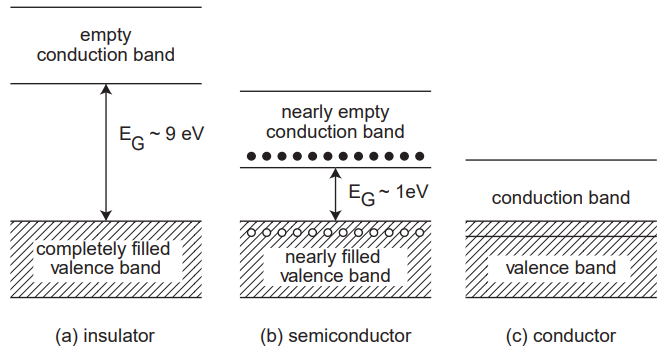
\includegraphics[width=0.48\textwidth]{figs/BandTheory.png}
%     \caption{Schematic illustration of the energy-band structure of insulators (a), semiconductors (b) and conductors (c) \cite{KolanoskiWermes}.}
%     \label{fig:bandTheory}
% \end{wrapfigure}
% By inserting impurities into the crystal structure of semiconductors the properties can be changed band gap can be reduced.
The properties of semiconductors can be changed by inserting impurities into the crystal structure.
If an atom with five electrons, called a donor, is inserted into an element with four electrons, an excessive conduction electron appears.
If an atom with three electrons, called an acceptor, is inserted into an element with three electrons, an excessive hole appears.
Semiconductors doped with donors are called n-doped while those doped with acceptors are called n-doped.
When both types of doped semiconductors are combined they form a diode.
% The electrons and the holes are drifting and recombining forming an electrical field between the two semiconductors.
Drifting and combining of $e^-/h^+$ forms an electrical field at the junction of the semiconductors which is called the depletion zone.
% In the depletion zone are no free charge carriers.
If an external positive voltage at the p side relative to the n side is applied this electrical field is weakened and current can flow which is called forward bias.
% This configuration is called forward bias.
In reverse bias, the electrical field is strengthened and the depletion zone increases. 
This configuration is used in detectors to measure ionizing particles. % it is used in semiconductor detectors so when an ionizing particle is moving through the diode the resulting charges can be measured.
            % Figure \ref{fig:geometries} shows the most important design configurations of semiconductor detectors.
            % \begin{wrapfigure}{r}{5.5cm}
            %     \centering
            %     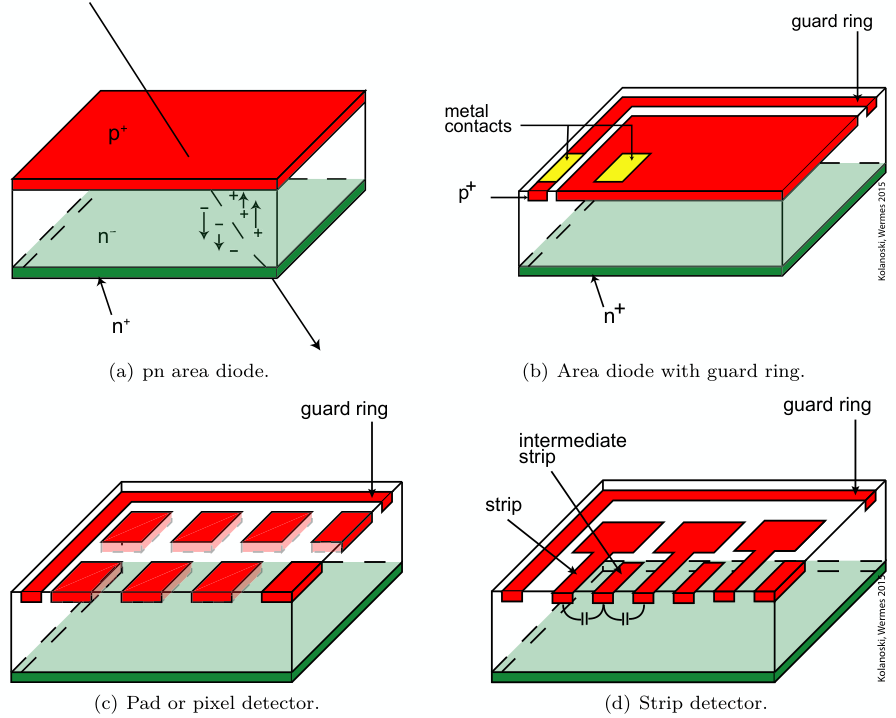
\includegraphics[width=0.4\textwidth]{figs/geometry.png}
            %     \caption{Schematic illustration of different types of geometries for semiconductor detectors \cite{KolanoskiWermes}.}
            %     \label{fig:geometries}
            % \end{wrapfigure}
            % The simplest design of such detectors is a pn area diode (a) consisting of a $\SI{300}{\micro\meter}$ thick p and an n-doped area that are combined to form a diode.
            % An additional guard ring can reduce the surface or leakage current thus reducing the electrical noise (b).
            % Dividing the area into strips of usually $\SIrange{50}{100}{\micro\meter}$ a strip detector (c) is created which can even give a space coordinate of detected particles.
            % Further dividing strip detectors into pad or pixel (at lengths below $\SI{100}{\micro\meter}$) detectors (d) can give two space coordinates but are much harder to read out than strip detectors.
            % The pixel detectors in ATLAS have sizes of $\SI{50}{\micro\meter}\times\SI{250}{\micro\meter}$.
\begin{figure}[H]
    \centering
    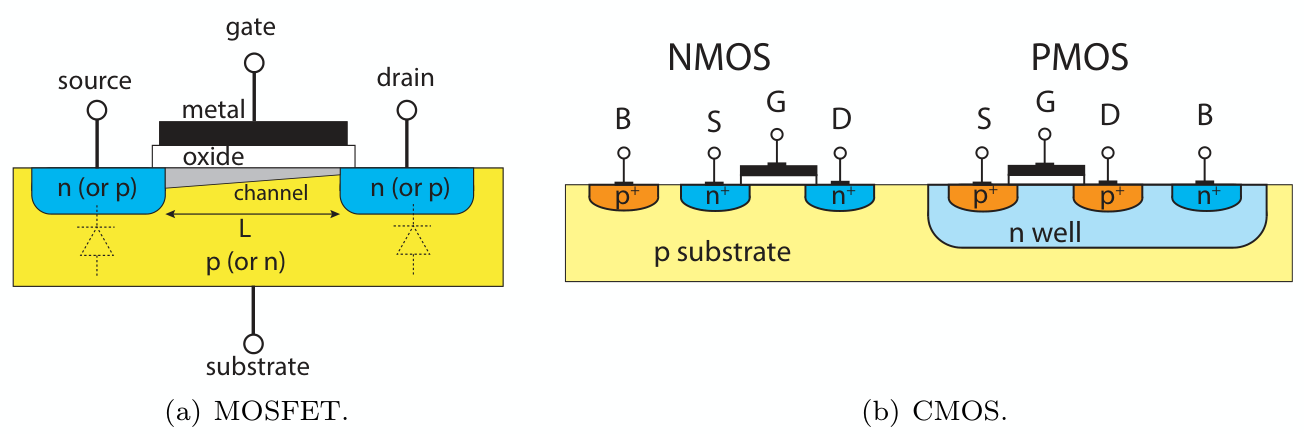
\includegraphics[width=0.69\textwidth]{figs/MOS.png}
    \caption{Schematic illustration of a MOSFET and a CMOS semiconductor \cite{KolanoskiWermes}.}
    \label{fig:MOStransition}
\end{figure}
The most used semiconductor detectors are complementary metal-oxide-semiconductors (CMOS) consisting of a part with a p-doped substrate and an n-doped drain terminal (NMOS) and a part with the reverse (PMOS).
Figure \ref{fig:MOStransition} a CMOS and a widely in field-effect transistor used semiconductor (MOSFET).

The simplest design of detectors is a pn area diode consisting of a $\SI{300}{\micro\meter}$ thick p and an n-doped area. % that are combined to form a diode.
An additional guard ring can reduce the electrical noise.
Dividing the area into strips or pixels ($\text{length}<\SI{100}{\micro\meter}$) yields one or even two spatial coordinates but increases the readout difficulty.
There are two different types to read out the information from the collection diodes.
Hybrid pixel sensors have the readout electronics on a different chip which is a laborious assembly and resides in a large material thickness, the sensor, however, can be separately optimized to the readout components.
Monolithic pixel sensors reduce their material by an entire order of magnitude but not all production lines are suited to produce such sensors.
As pixel detectors are used to reconstruct traces for example in the ATLAS Experiment due to their good resolution with an uncertainty of $\sigma_x=\sfrac{\text{pitch}}{\sqrt{12}}$ \cite{Tom}, they are placed closest to the collision vertex where a lot of charged particles pass through them causing damage to the detector substrate.
Such radiation damage can cause a change in effective doping concentration leading to deactivated donor or acceptor atoms.
They can furthermore cause trapping where $e^-/h^+$ are trapped in defects of the crystal structure and are released later.
These defects can form energy levels that excite $e^-/h^+$ easier and cause a flow in current. % which is called leakage current.
Radiation damage can be reduced by cooling.
\begin{wrapfigure}{l}{7.5cm}
    \centering
    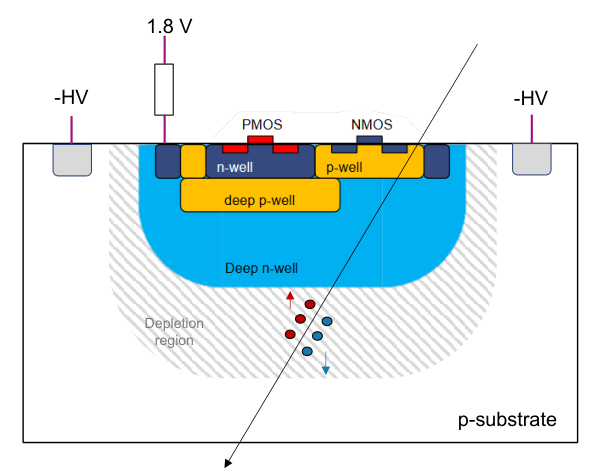
\includegraphics[width=0.5\textwidth]{figs/MightyPix.png}
    \caption{Schematic illustration of a MightyPix \cite{MightyPix}.}
    \label{fig:MightyPix}
\end{wrapfigure}
A track is reconstructed by forming groups of measurement points, called tracklets which require a good spatial and time resolution of the pixel detectors.
In each of the tracklets every possible combination is built but only those that point to the interacting point are accepted forming a track when a series of tracklets match.
% A track is reconstructed when a series of tracklets match.
An application of pixel detectors is given in the example of MightyPix, a design sketch of possible pixel detectors used in the second upgrade of the LHC.
Their final requirements for the upgrade include a time resolution of $<\SI{3}{\nano\second}$, and a pixel size of $~\SI{50}{\micro\meter}\times\SI{150}{\micro\meter}$. % and power consumption of $<\SI{0.15}{\watt\per\centi\meter\squared}$ allowing for a good resolution.
Semiconductor detectors in the form of pixel detectors provide good time and space resolution which is why particle detectors are indispensable without them.
But the implementation of pixel detectors brings new challenges like the power distribution or the cooling of the detectors.

% \begin{figure}
%     \centering
%     \begin{subfigure}[b]{.48\linewidth}
%         \includegraphics[width=\linewidth]{figs/Bandtheory.png}
%         \caption{Schematic illustration of different types of geometries for semiconductor detectors \cite{KolanoskiWermes}.}
%         \label{fig:geometries}
%     \end{subfigure}
%     \begin{subfigure}[b]{.48\linewidth}
%         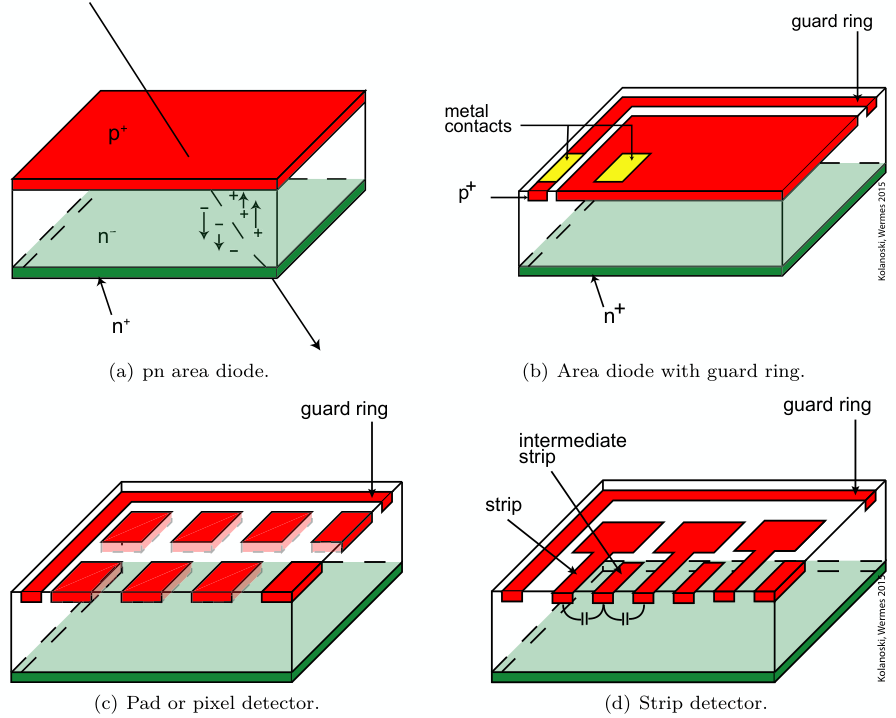
\includegraphics[width=\linewidth]{figs/geometry.png}
%         \caption{Schematic illustration of different types of geometries for semiconductor detectors \cite{KolanoskiWermes}.}
%         \label{fig:geometries}
%     \end{subfigure}
%     \label{fig:picsSemiconductors}
%     \caption{}
% \end{figure}